\chapter{Stand der Forschung}
\section{Einführung in die künstliche Intelligenz}
TODO: Quelle (wie unten?)
Intelligenz ist nicht konkret definiert ist. Der Begriff bezieht sich auf den Menschen. Der Begriff "künstliche Intelligenz" bezieht sich auf Rechner. Hier ist der Teil \textit{künstlich} des Begriffs definiert: Die künstliche Intelligenz zielt darauf ab, intelligente Rechner zu programmieren. Im diesem Kontext redet man auch oft von intelligenten Agenten. Der Teil \textit{Intelligenz} des Begriffs ist jedoch auch in diesem Zusammenhang nicht definiert und verweist lediglich auf den Begriff im menschlichen Kontext.
Einige intelligente Agenten sind bereits allgemein bekannt:
\begin{itemize}
\item Taschenrechner
\item Schachcomputer
\item Suchmaschinen (z.B. Google und auch deren Übersetzer)
\item dynamische Spamfilter 
\item lernende Roboter (Saugroboter, die ihre Umgebung erkunden) 
\end{itemize}

Die Robotik macht sich also, wie oben aufgeführt intelligente Systeme zu nutze. Es gibts jedoch auch andere, nicht physikalisch vorhanden Systeme, die intelligente Agenten einsetzt (Spamfilter, ...). Es existiert somit eine Kategorisierung, die nach physikalischem Vorhandensein einteilt:
\begin{itemize}
\item Roboter
\item und Bots
\end{itemize} 
Bots sind nur logisch vorhanden und Roboter auch physikalisch. Beide nutzen intelligente Agenten. 


\begin{figure}%[h!]
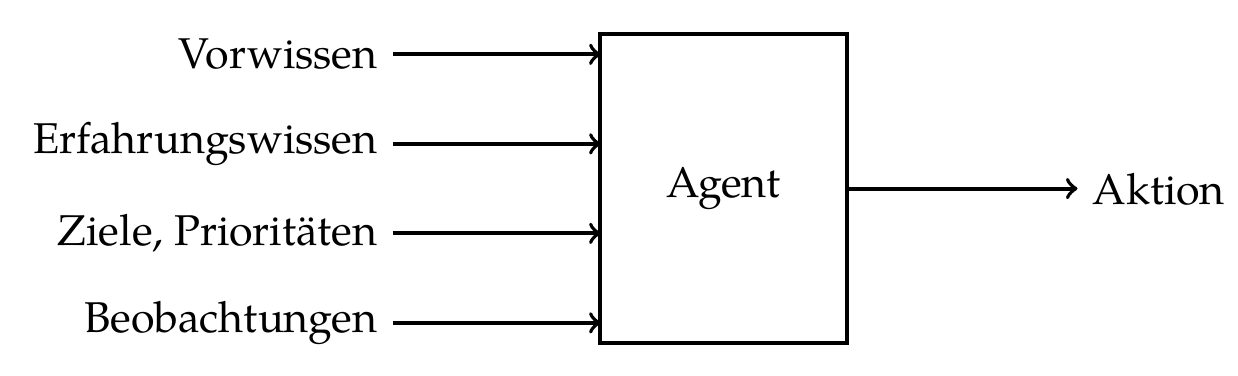
\includegraphics[scale=0.3]{bilder/agent} 
\caption{Agenten \cite{Schauss}}
\label{Agenten}
\end{figure}


Nach \cite{Russel10} kann man die künstliche Intelligenz in vier Klassen einteilen
\begin{enumerate}
\item menschliches Handeln
\item menschliches Denken
\item rationales Denken
\item rationales Handeln
\end{enumerate}
Diese Kategorien sind in den folgenden Unterkapiteln genauer aufgeführt, wobei die ersten beiden Kategorien sich an dem Menschen orientieren und die letzten beiden an mathematischen Modellen. 

\subsection{Menschliches Handeln}
Ein Ziel der künstlichen Intelligenz hier ist, menschliches Handeln mithilfe von Robotern nachzuahmen. Dies können Aspekte sein, die beispielsweise momentan nur für Menschen möglich sind oder in denen der Mensch Computern überlegen ist.    

\subsection{Menschliches Denken}
Um künstlich das menschliche Denken nachzubilden, muss  man erst einmal verstehen, wie der Mensch überhaupt denkt. Dies ist nicht einfach herauszufinden. Modelle die, die Verhaltensforscher durch Versuche aufstellen,  können hier helfen. Die Modelle können Systeme sein. Ein System ist in diesem Kontext gekennzeichnet durch eine Ein- und eine Ausgabe. Gleichen nun Ein- und Ausgabe des Systems denen dem menschlichen Denken, ist das ein positives Indiz für die Eignung des Modells.

Wesentliche Fragen auf diesem Gebiet sind:
\begin{itemize}
\item Bildverarbeitung und Gestenerkennung beim Menschen
\item Sprachverarbeitung von menschlicher Sprache
\end{itemize}    

Man verfolgt hier das Ziel, kognitiv adäquate Systeme zu bauen. Ein Taschenrechner ist zum Beispiel nicht kognitiv adäquat zum Menschen. Er rechnet auf eine andere Art und Weise die Addition zweier Zahlen aus.
\subsection{Rationales Denken}
Ein großer Bestandteil des rationalen Denkens ist die Logik. Die Logik ist klassischerweise formal. Um nun aus logischen Zusammenhängen für einen Informationsgewinn zu nutzen, kann man sich an der Deduktion bedienen. 

\begin{itemize}
\item Alles Hunde können schnell rennen.
\item Ben ist ein Hund.
\end{itemize}
$\rightarrow$ Ben ist schnell.

Kann ein Sachverhalt als logische Aussage formalisiert werden, so kann man durch beispielsweise die Deduktion ein intelligentes System implementieren. 

\subsection{Rationales Handeln}
Systeme, die rational Handeln verfolgen im Idealfall autonom und flexibel ein Ziel. Flexibel meint, dass das System auch nach geänderten äußerlichen Einflüssen immer noch in der Lage ist, das Ziel zu identifizieren und es weiterhin zu verfolgen. Es handelt sich hierbei um die oben genannten Agenten. Das Ziel, dass sie verfolgen ist hierbei das Maximum aus dem rationalen Blickwinkel. Menschliche Eingenschaften miteinzubeziehen ist auch möglich, erhöht jedoch den Grad der Komplexität. Es ist wesentlich einfacher logische und mathematische Sachverhalte zu implementieren ohne menschliche Aspekte zu beachten.

\section{Maschinelles Lernen}
Da es problematisch ist eine ausreichend gute Lösung für einen intelligenten Agenten beim Implementieren zu realisieren, behilft man sich anderweitig. Man wendet Verfahren an, bei denen man den Agenten selber, also die Maschine, lernen lässt. Dies nennt sich \textit{maschinelles Lernen}.
Im Rahmen dieser Ausarbeitung werden Bayes'sche Netze genauer betrachtet. Sie helfen in Kombination mit maschinellem Lernen komplexe Probleme in der Informatik zu vereinfachen. Somit ist es möglich, derartige Probleme mit gegebenen Rechenressourcen in einem angemessenen Zeitraum zu lösen. 

TODO Quelle: [Bayes] --> sicher??




